\documentclass{article}

\usepackage{amsmath}

\usepackage{bm}

\usepackage{physics}

\usepackage{graphicx}
\usepackage{epstopdf}
\graphicspath{{img/}}

\everymath{\displaystyle}

\begin{document}

\title{Quantum physics: I set of exercises - Solutions}
\author{Giancarlo Fissore}
\date{January 2015}
\maketitle

\section{Oscillating wavepacket}

\subsection{Time evolution of \(\psi\)}
To compute the time evolution of the state

\begin{equation}
\psi(x,0) = N_0 e^{-\frac{1}{2} \alpha^2 (x-a)^2}
\end{equation}

we can project the state on the eigenstates of the energy

\begin{equation}
\psi(x,0) = \sum_{n} \braket{\psi_n}{\psi} \ket{\psi_n} = \int dx' \psi_n^*(x') \psi(x') \psi_n(x)
\end{equation}

and then add the time evolution phase factor for each eigenstate

\begin{equation}
\psi(x,t) = \sum_{n} \int dx' \psi_n^*(x') \psi(x') \psi_n(x) e^{-i \frac{E_n}{\hbar} t}
\end{equation}

The expression of the eigenstates of the energy for the harmonic oscillator is

\begin{equation}
\psi_n(x) = \frac{\alpha^{\frac{1}{2}}}{\pi^{\frac{1}{4}} \sqrt{2^n n!}} e^{-\frac{(\alpha x)^2}{2}} H_n(\alpha x)
\end{equation}

where \( H_n(x) \) is the \(n^{th}\) degree Hermite polynomial, whose definition is given by

\begin{equation}
H_n(x) = (-1)^n e^{x^2} \frac{d^n}{dx^n} e^{-x^2}
\end{equation}

First of all, let's compute the projection of \( \psi \) on the eigenstate \( \psi_n \)

\begin{align}
& \int dx \, \psi_n^*(x) \psi(x) = \nonumber \\
& = \frac{(-1)^n N_0 \alpha^{\frac{1}{2} - n}}{\pi^{\frac{1}{4}} \sqrt{2^n n!}} \int dx \, e^{\frac{(\alpha x)^2}{2}} \frac{d^n}{dx^n} \left[ e^{-(\alpha x)^2} \right] e^{-\frac{\alpha^2(x-a)^2}{2}} \nonumber \\
& = \frac{(-1)^n N_0 \alpha^{\frac{1}{2} - n}}{\pi^{\frac{1}{4}} \sqrt{2^n n!}} e^{-\frac{1}{2} \alpha^2 a^2} \int dx \, \frac{d^n}{dx^n} \left[ e^{-(\alpha x)^2} \right] e^{a \alpha^2 x} \nonumber \\
& = k \int dx \, \frac{d^n}{dx^n} \left[ e^{-(\alpha x)^2} \right] e^{a \alpha^2 x} \nonumber \\
& = k \left\{ \left[ \frac{d^{n-1}}{dx^{n-1}} \left[ e^{-(\alpha x)^2} \right] e^{a\alpha^2x} \right]_{-\infty}^{\infty} \right\} - k \int dx \, \frac{d^{n-1}}{dx^{n-1}} \left[ e^{-(\alpha x)^2} \right] a \alpha^2 e^{a \alpha^2 x} \nonumber \\
& = - k \left\{ \left[ \frac{d^{n-2}}{dx^{n-2}} \left[ e^{-(\alpha x)^2} \right] a \alpha^2 e^{a\alpha^2x} \right]_{-\infty}^{\infty} \right\} + k \int dx \, \frac{d^{n-2}}{dx^{n-2}} \left[ e^{-(\alpha x)^2} \right] (a \alpha^2)^2 e^{a \alpha^2 x} \nonumber \\
& = \ldots = k (-1)^n (a \alpha^2)^n \int dx \, e^{-\alpha^2 (x^2 + ax)} \nonumber \\
& = k (-1)^n (a \alpha^2)^n \int dx \, e^{-\alpha^2 (x^2 + ax)} \frac{\sqrt{\pi}}{\alpha} e^{\frac{a^2 \alpha^2}{4}} \nonumber \\
& = \frac{N_0 \pi^{\frac{1}{4}}}{\sqrt{2^n n!}} \alpha^{-\frac{1}{2}+n} a^n e^{-\frac{a^2 \alpha^2}{4}}
\end{align}

The explicit expression of \( E_n \) is

\begin{equation}
E_n = \hbar \omega \left( n + \frac{1}{2} \right)
\end{equation}

and the time evolution of \( \psi \) is given by

\begin{align}
\psi(x,t) & = \sum_n \int dx' \, \psi_n(x')_* \psi_n(x') \psi_n(x) e^{-i \frac{E_n}{\hbar}t} \nonumber \\
& = N_0 e^{-\frac{(\alpha x^2)}{2}} e^{-\frac{(\alpha a)^2}{4}} e^{-i \frac{\omega}{2} t} \sum_n \frac{\alpha^n a^n}{2^n n!} H_n(\alpha x) e^{-i \omega n t} \nonumber \\
& = N_0 e^{-\frac{(\alpha x^2)}{2}} e^{-\frac{(\alpha a)^2}{4}} e^{-i \frac{\omega}{2} t} \sum_n \frac{H_n(\alpha x)}{n!} \left( \frac{\alpha a e^{-i \omega n t}}{2} \right)^n
\end{align}

To proceed with the computation, we report the expression of the generating function of Hermite polynomials

\begin{equation}
\sum_n \frac{H_n(x)}{n!} t^n = e^{2xt-t^2}
\end{equation}

Then we have

\[
\sum_n \frac{H_n(\alpha x)}{n!} \left( \frac{\alpha a e^{-i\omega t}}{2} \right)^n = e^{\frac{\alpha^2 a}{2} x e^{-i \omega t} - \frac{\alpha^2 a^2}{4}e^{-2i \omega t}}
\]

and \( \psi(x,t) \) is

\begin{equation}
\psi(x,t) = N_0 e^{-\frac{\alpha^2 a^2}{4}\left( 1 + e^{-2i \omega t} \right)} e^{-i \frac{\omega}{2} t} e^{-\frac{(\alpha x^2)}{2}} e^{\alpha^2 a x e^{-i \omega t}}
\end{equation}

\subsection{Computation of density}
To compute the density

\begin{equation}
\rho(x,t) = |\psi(x,t)|^2
\end{equation}

we first rewrite \( \psi(x,t) \) separating complex and real exponentials

\begin{align}
\psi(x,t) & = N_0 e^{-\frac{\alpha^2 a^2}{4}\left(1 + cos(2\omega t) - i \, sin(2 \omega t) \right)} e^{-i \frac{\omega}{2} t} e^{-\frac{(\alpha x)^2}{2}} e^{\alpha^2 a x (cos(\omega t) - i \, sin(\omega t))} \nonumber \\
& = N_0 e^{-\frac{\alpha^2 a^2}{4}\left(1 + cos(2\omega t) \right)} e^{-\frac{(\alpha x)^2}{2}} e^{\alpha^2 a x \, cos(\omega t)} e^{-i \alpha^2 a x \, sin(\omega t)} e^{i \frac{\alpha^2 a^2}{4}sin(2\omega t)} e^{-i \frac{\omega}{2} t}
\end{align}

then it is easy to see that the comlex exponentials cancel out and the result is given by the square of real exponentials

\begin{align}
\rho(x,t) & = |\psi(x,t)|^2 = |\psi^*(x,t) \psi(x,t)|^2 = \nonumber \\
& = N_0 e^{-\frac{\alpha^2 a^2}{2}\left(1 + cos(2\omega t) \right)} e^{-(\alpha x)^2} e^{2 \alpha^2 a x \, cos(\omega t)}
\end{align}

\section{3D square well}

\subsection{Radial Schroedinger equation}
Because of the spherical simmetry of the potential, it is a good choice to use spherical coordinates in solving the problem. We recall the expression of the laplacian in spherical coordinates

\begin{equation}
\label{eq:laplacian_spher}
\nabla^2 = \frac{1}{r^2} \left( \frac{\partial}{\partial r} r^2 \frac{\partial}{\partial r} + \frac{1}{sin\theta} \frac{\partial}{\partial \theta} sin\theta \frac{\partial}{\partial \theta} + \frac{1}{sin^2\theta} \frac{\partial^2}{\partial \varphi^2} \right)
\end{equation}

The hamiltonian of the problem is

\begin{equation}
\label{eq:hamiltonian_spher}
H = \frac{p^2}{2m} + V(r) = -\frac{\hbar^2 \nabla^2}{2m} + V(r)
\end{equation}

and the time-independent Schroedinger equation is

\begin{equation}
\label{eq:schroedinger_ti}
H\Psi(\bm{r}) = E\Psi(\bm{r})
\end{equation}

Eq. \eqref{eq:laplacian_spher} and \eqref{eq:hamiltonian_spher} suggest the existence of factorized solutions for \eqref{eq:schroedinger_ti}. Moreover, because of the spherical simmetry of the potential, the hamiltonian of the problem commutes with the angular momentum operators \(L^2\) and \(L_{z}\) whose eigenfunctions are the spherical harmonics \(Y_{l}^m(\theta,\phi)\). The solutions of the problem will then have the following form:

\begin{equation}
\label{eq:factorized_psi}
\Psi(\bm{r}) = \varphi(r) Y_{l}^m(\theta,\phi)
\end{equation}

To solve for the radial component it is then necessary to recall the following equations:

\begin{equation}
\label{eq:p2_decomposed}
p^2 = p_{r}^2 + \frac{L^2}{r^2}
\end{equation}

\begin{equation}
\label{eq:p_radial}
p_{r} = -i\hbar \left( \frac{\partial}{\partial r} + \frac{1}{r} \right)
\end{equation}

\begin{equation}
\label{eq:L2_eigenvalues}
L^2 Y_{l}^m(\theta, \phi) = \hbar^2 l(l+1) Y_{l}^m(\theta, \phi)
\end{equation}

Using \eqref{eq:p2_decomposed}, \eqref{eq:factorized_psi} and \eqref{eq:L2_eigenvalues} 
it is easy to show that the time-independent Schroedinger equation \eqref{eq:schroedinger_ti} becomes

\begin{equation}
\left[ \frac{1}{2m} \left( p_{r}^2 + \frac{\hbar^2 l(l+1)}{r^2} \right) + V(r) \right] \varphi(r) Y_{l}^m(\theta, \phi) = E \varphi(r) Y_{l}^m(\theta, \phi)
\end{equation}

Canceling out the spherical harmonics and plugging in eq. \eqref{eq:p_radial} we obtain the radial Schroedinger equation

\begin{equation}
\label{eq:schroedinger_radial}
\frac{d^2 \varphi}{dr^2} + \frac{2}{r} \frac{d\varphi}{dr} + \left\{ \frac{2m}{\hbar^2} \left[ E - V(r) \right] - \frac{l \left(l+1 \right)}{r^2} \right\} \varphi = 0
\end{equation}

As the value \(l\) appears in the equation, the value of the solution will depend on \(l\):

\[ \varphi(r) \Rightarrow \varphi_l(r) \]

\subsection{Solution to the radial Schroedinger equation}
For \( \left| \bm{r} \right| = r < a \) we have \( V(r) = -V_0 \) and the radial Schroedinger equation \eqref{eq:schroedinger_radial} takes the form

\begin{equation}
\label{eq:rs_inside_sphere}
\left[ \frac{d^2}{dr^2} + \frac{2}{r} \frac{d}{dr} - \frac{l \left(l+1 \right)}{r^2} \right] \varphi_{l,1} = - \frac{2m(E+V_0)}{\hbar^2} \varphi_{l,1} = -k_1^2 \varphi_{l,1}
\end{equation}

\begin{equation}
k_1 = \sqrt{\frac{2m(E+V_0)}{\hbar^2}}, \quad k_1 > 0 \quad (E<0)
\end{equation}

Making the change of variable \( r \rightarrow z = k_1r \) we can recognize eq. \eqref{eq:rs_inside_sphere} to be the Bessel spherical differential equation with argument \(z = k_1 r\), for which we choose the following solution

\begin{equation}
\varphi_{l,1}(k_1r) = A j_l(k_1r) + B \eta_l(k_1r)
\end{equation}

As \( \eta_l \) is divergent for \( r \rightarrow 0 \), for the solution to be physically acceptable we must have

\begin{equation}
B = 0 \quad \Rightarrow \quad \varphi_{l,1}(k_1r) = A j_l(k_1r)
\end{equation}

For \( \left| \bm{r} \right| = r > a \) we have \( V(r) = 0 \) and the radial Schroedinger equation \eqref{eq:schroedinger_radial} takes the form

\begin{equation}
\label{eq:rs_outside_sphere}
\left[ \frac{d^2}{dr^2} + \frac{2}{r} \frac{d}{dr} - \frac{l \left(l+1 \right)}{r^2} \right] \varphi_{l,1} = - \frac{2mE}{\hbar^2} \varphi_{l,1} = - i^2 k_2^2 \varphi_{l,1} = k_2^2 \varphi_{l,1}
\end{equation}

\begin{equation}
k_2 = \sqrt{\frac{-2mE}{\hbar^2}}, \quad k_2 > 0 \quad (E<0)
\end{equation}

Making the change of variable \( r \rightarrow z = i k_2 r \) we can recognize eq. \eqref{eq:rs_outside_sphere} to be the Bessel spherical differential equation with argument \(z = i k_2 r\). Given that the argument is purely imaginary and we care about the behaviour for \( r \rightarrow \infty \), the right solution to choose is a linear combination of Hankel functions

\begin{equation}
\varphi_{l,2}(ik_2r) = C h_l^1(ik_2r) + D h_l^2(ik_2r)
\end{equation} 

whose asymptotic behaviour for \( r \rightarrow \infty \) is given by

\begin{equation}
h_l^1(ik_2r) \sim -(-i)^l \frac{e^{-k_2r}}{k_2r} \rightarrow 0
\end{equation}

\begin{equation}
\label{eq:h2_asymptotic}
h_l^2(ik_2r) \sim i^l \frac{e^{k_2r}}{k_2r} \rightarrow \infty
\end{equation}

Given eq. \eqref{eq:h2_asymptotic}, for the solution to be physically meaningful we must have

\begin{equation}
D = 0 \quad \Rightarrow \quad \varphi_{l,2}(ik_2r) = C h_l^1(ik_2r)
\end{equation}

Of course the total wave function must be continuous and with continuous first derivative, thus we impose the following boundary conditions

\begin{equation}
\varphi_{l,1}(k_1a) = \varphi_{l,2}(ik_2a)
\end{equation}

\begin{equation}
\varphi_{l,1}'(k_1a) = \varphi_{l,2}'(ik_2a)
\end{equation}

Substituting the expressions for \( \varphi_l \) into the boundary conditions we get the following system

\begin{equation}
  \begin{cases}
    A j_l(k_1a) & = C h_l^1(ik_2a) \\
    A k_1 j_l'(k_1a) & = C i k_2 {h_l^1}'(ik_2a)
  \end{cases}
\end{equation}

Solving the first equation for \( A \) and substituting into the second, we obtain

\begin{equation}
C \left( k_1 \frac{h_l^1(ik_2a)}{j_l(k_1a)} j_l' - i k_2 {h_l^1}'(ik_2a) \right) = 0
\end{equation}

Solutions with \( C = 0 \) are trivial (wave function null everywhere) then to get the allowed values of energy we are interested in solving the following equation

\begin{equation}
\label{eq:log_derivative}
k_1 \frac{j_l'(k_1a)}{j_l(k_1a)} = i k_2 \frac{{h_l^1}'(ik_2a)}{h_l(ik_2a)}
\end{equation}

\subsection{ \( l = 0 \) }

With \( l= 0 \) we have

\begin{equation}
j_0(z) = \frac{sin(z)}{z}
\end{equation}

\begin{equation}
\eta_0(z) = - \frac{cos(z)}{z}
\end{equation}

\begin{equation}
j_0'(z) = \frac{cos(z)}{z} -  \frac{sin(z)}{z^2}
\end{equation}

\begin{equation}
\eta_0'(z) = \frac{sin(z)}{z} + \frac{cos(z)}{z^2}
\end{equation}

Then the first member of eq. \eqref{eq:log_derivative} is

\begin{align}
k_1 \frac{j_0'(k_1a)}{j_0(k_1a)} & = k_1 \left( \frac{cos(k_1a)}{k_1a} - \frac{sin(k_1a)}{(k_1a)^2} \right) \frac{k_1a}{sin(k_1a)} \nonumber \\
& = k_1 \left( \frac{cos(k_1a)}{sin(k_1a)} - \frac{1}{k_1a} \right) \nonumber \\
& = k_1 cot(k_1a) - \frac{1}{a}
\end{align}

while the second is

\begin{align}
ik_2a \frac{h_0'(ik_2a)}{h_0(ik_2a)} & = ik_2 \frac{j_0'(ik_2a) + i \eta_0'(ik_2a)}{j_0(ik_2a) + i\eta_0(ik_2a)} \nonumber \\
& = ik_2 \frac{\frac{cos(ik_2a)}{ik_2a} - \frac{sin(ik_2a)}{(ik_2a)^2} + i \left( \frac{sin(ik_2a)}{ik_2a} + \frac{cos(ik_2a)}{(ik_2a)^2} \right)}{\frac{sin(ik_2a)}{ik_2a} -i \frac{cos(ik_2a)}{ik_2a}} \nonumber \\
& = \frac{1}{a} \frac{ik_2a \, cos(ik_2a) - sin(ik_2a) - k_2a \, sin(ik_2a) + i \, cos(ik_2a)}{sin(ik_2a) - i \, cos(ik_2a)} \nonumber \\
& = \frac{1}{a} \frac{(1+k_2a) \left[ i \, cos(ik_2a) - sin(ik_2a) \right]}{-i \left[ cos(ik_2a) + i \, sin(ik_2a) \right]} \nonumber \\
& = \frac{1}{a} i^2 (1 + k_2a) = -k_2 - \frac{1}{a}
\end{align}

Finally, eq. \eqref{eq:log_derivative} becomes

\begin{equation}
k_1a \, cot(k_1a) = -k_2a
\end{equation}

\subsection{\(l=1\)}

For \( l = 1 \) we have

\begin{equation}
j_1(z) = \frac{sin(z)}{z^2} - \frac{cos(z)}{z}
\end{equation}

\begin{equation}
\eta_1(z) = - \frac{cos(z)}{z^2} - \frac{sin(z)}{z}
\end{equation}

\begin{equation}
j_1'(z) = \left( \frac{1}{z} - \frac{2}{z^3} \right) sin(z) + 2 \frac{cos(z)}{z^2}
\end{equation}

\begin{equation}
\eta_0'(z) = \left( \frac{2}{z^3} - \frac{1}{z} \right) cos(z) + 2 \frac{sin(z)}{z^2}
\end{equation}

The first member of eq. \eqref{eq:log_derivative} results

\begin{align}
k_1 \frac{j_1'(k_1a)}{j_1(k_1a)} & = k_1 \frac{ \left( \frac{1}{k_1a} - \frac{2}{(k_1a)^3} \right) sin(k_1a) + 2 \frac{cos(k_1a)}{(k_1a)^2}}{\frac{sin(k_1a)}{(k_1a)^2} - \frac{cos(k_1a)}{k_1a}} \nonumber \\
& = k_1 \left( \frac{(k_1a)^2-2}{(k_1a)^3} sin(k_1a) + 2 \frac{cos(k_1a)}{(k_1a)^2} \right) \frac{(k_1a)^2}{sin(k_1a)-k_1a \, cos(k_1a)} \nonumber \\
& = \frac{1}{a} \frac{\left[ (k_1a)^2 - 2 \right] sin(k_1a) + 2k_1a \, cos(k_1a)}{sin(k_1a) - k_1a \, cos(k_1a)}
\end{align}

and the second member is

\begin{align}
& ik_2 \frac{h_1'(ik_2a)}{h_1(ik_2a)} = ik_2 \frac{j_1'(ik_2a) + i \eta_1'(ik_2a)}{j_1(ik_2a) + i \eta_1(ik_2a)} \nonumber \\
& = ik_2 \frac{\left( \frac{1}{ik_2a} - \frac{2}{(ik_2a)^3} \right) sin(ik_2a) + 2 \frac{cos(ik_2a)}{(ik_2a)^2} + i \left( \frac{2}{(ik_2a)^3} - \frac{1}{ik_2a} \right) cos(ik_2a) + 2i \frac{sin(ik_2a)}{(ik_2a)^2}}{\frac{sin(ik_2a)}{(ik_2a)^2} - \frac{cos(ik_2a)}{ik_2a} - i \frac{cos(ik_2a)}{(ik_2a)^2} - i \frac{sin(ik_2a)}{ik_2a}} \nonumber \\
& = ik_2(ik_2a)^2 \frac{\frac{(ik_2a)^2-2}{(ik_2a)^3}sin(ik_2a) + 2 \frac{cos(ik_2a)}{(ik_2a)^2}+i \frac{2-(ik_2a)^2}{(ik_2a)^3}cos(ik_2a)+2i \frac{sin(ik_2a)}{(ik_2a)^2}}{sin(ik_2a) - ik_2a \, cos(ik_2a) -i \, cos(ik_2a) + k_2a \, sin(ik_2a)} \nonumber \\
& = \frac{sin(ik_2a) \left[(ik_2a)^2 - 2 - 2k_2a \right] - i \, cos(ik_2a) \left[ (ik_2a)^2 -2 - 2k_a \right]}{(1+k_2a) \left[ sin(ik_2a) - i \, cos(ik_2a) \right]} \nonumber \\
& = \frac{1}{a} \frac{(k_2a)^2 + 2 + 2k_2a}{1+k_2a}
\end{align}

The equation then looks

\begin{equation}
\frac{\left[ (k_1a)^2 - 2 \right] sin(k_1a) + 2k_1a \, cos(k_1a)}{sin(k_1a) - k_1a \, cos(k_1a)} = \frac{(k_2a)^2 + 2 + 2k_2a}{1+k_2a}
\end{equation}

\subsection{Emergence of bound states}
In this section we will derive, for arbitrary \( l \), the minimum value of \( V_0a^2 \) for which the first bound state emerges. In such situation the energy approches 0 and we have

\begin{equation}
E \rightarrow 0
\end{equation}

\begin{equation}
k_1 \rightarrow \frac{\sqrt{2mV_0}}{\hbar^2}
\end{equation}

\begin{equation}
k_2 \rightarrow 0
\end{equation}

Recalling the following relations for the spherical Bessel functions

\begin{equation}
\label{eq:bessel_derivative}
\varphi_l'(z) = \frac{l}{z} \varphi_l(z) - \varphi_{l+1}(z) = \varphi_{l-1}(z) - \frac{l+1}{z} \varphi_l(z)
\end{equation}

\begin{equation}
j_l(z) \sim \frac{z^l}{(2l+1)!!}, \quad z \rightarrow 0
\end{equation}

\begin{equation}
\eta_l(z) \sim -\frac{(2l-1)!!}{z^{l+1}}, \quad z \rightarrow 0
\end{equation}

and making the change of variable \( z = ik_2r \) we can simplify the second member of eq. \eqref{eq:log_derivative} to obtain (as \(z \rightarrow 0 \))

\begin{align}
\frac{z}{a} \frac{h_l'(z)}{h_l(z)} & = \frac{z}{a} \left(\frac{l}{z} - \frac{h_{l+1}(z)}{h_l(z)} \right) \nonumber \\
& = \frac{l}{a} - \frac{z}{a} \frac{h_{l+1}(z)}{h_l(z)} \nonumber \\
& = \frac{l}{a} - \frac{z}{a} \frac{j_{l+1}(z) + i\eta_{l+1}(z)}{j_l(z)+i\eta_l(z)} \nonumber \\
& = \frac{l}{a} - \frac{z}{a} \frac{z^{2l+3}-i(2l+2)!!(2l+1)!!}{(2l+2)!!z^{l+2}} \frac{(2l+1)!!z^{l+1}}{z^{2l+1}-i(2l+1)!!(2l-1)!!} \nonumber \\
& = \frac{1}{a} (2l+1)
\end{align}

Eq. \eqref{eq:log_derivative} then becomes

\begin{equation}
\label{eq:asymptotic_log_derivative}
\frac{j_l'(k_1a)}{j_l(k_1a)} = - \frac{l+1}{k_1a} \quad \Rightarrow \quad j_l'(k_1a) = - \frac{l+1}{k_1a} j_l(k_1a)
\end{equation}

and comparing \eqref{eq:asymptotic_log_derivative} with \eqref{eq:bessel_derivative} we must have

\begin{equation}
j_{l-1}(k_1a) = 0
\end{equation}

Naming by \( z_{1,l} \) the first zero of the \( l^{th} \) Bessel function, we can easily obtain the minimum value of \(V_0a^2 \) for which a bound state emerges

\begin{equation}
k_1a = \frac{\sqrt{2mV_0}}{\hbar^2}a = z_{1,l} \quad \Rightarrow \quad V_0a^2 = \frac{\hbar^2}{2m}z_{1,l}^2
\end{equation}

As \(z_{1,l} \) is increasing with \(l\), we can conclude that \(V_0a^2\) is increasing monotonically with \(l\).

\section{Double well potential}

\subsection{Schroedinger equation and boundary conditions}
First of all, the Schroedinger equation for the problem is presented below.

For \(\left|x\right| < a\):

\begin{equation}
\label{eq:schr1}
-\frac{\hbar^2}{2m}\psi_{1}(x) + V_{0}\psi_{1}(x) = E\psi_{1}(x)
\end{equation}

For \(a < \left|x\right| < L\):

\begin{equation}
\label{eq:schr2}
-\frac{\hbar^2}{2m}\psi_{2}(x) = E\psi_{2}(x)
\end{equation}

For \(\left|x\right| > L\):

\begin{equation}
\label{eq:schr3}
-\frac{\hbar^2}{2m}\psi_{3}(x) = E\psi_{3}(x)
\end{equation}

Obviously the wave function for \(\left|x\right| > L\) must be null, as the potential is infinite in such region, thus we have

\begin{equation}
\psi_{3}(x) = 0
\end{equation}

The total wave function must be continuous and with continuous first derivative, thus we impose the following boundary conditions

\begin{equation}
\label{eq:continuity}
\psi_{1}(a) =  \psi_{2}(a)
\end{equation}

\begin{equation}
\psi_{1}(-a) =  \psi_{2}(-a)
\end{equation}

\begin{equation}
\label{eq:continuity_derivative}
\psi_{1}'(a) =  \psi_{2}'(a)
\end{equation}

\begin{equation}
\psi_{1}'(-a) =  \psi_{2}'(-a)
\end{equation}

\begin{equation}
\label{eq:null_bound}
\psi_{2}(L) =  \psi_{3}(L) = 0
\end{equation}

\subsection{Solutions with definite parity}
To simplify the treatment of the problem, it is useful to note that because of the simmetry of the potential the Hamiltonian is commuting with the parity operator. This is easily shown below

\begin{align*}
[H, \hat{\pi}] \Psi(x) & = H \hat{\pi} \Psi(x) - \hat{\pi} H \Psi(x) \\ 
  & = \left(-\frac{\hbar^2}{2m} + V(x)\right)\Psi(-x) -  \hat{\pi} \left(-\frac{\hbar^2}{2m} + V(x)\right)\Psi(x) \\ & = \left(-\frac{\hbar^2}{2m} + V(x)\right)\Psi(-x) -  \left(-\frac{\hbar^2}{2m} + V(-x)\right)\Psi(-x)
\end{align*}

\begin{equation}
\label{eq:parity_commutation}
V(x) = V(-x) \Rightarrow \left[H,\hat{\pi} \right] = 0
\end{equation}

Applying \(\hat{\pi}\) to one of its eigenfunctions twice, the original function is retrieved

\begin{equation}
\hat{\pi}^2f(x) = \hat{\pi}f(-x) = f(x)
\end{equation}

Therefore, the operator \(\hat{\pi}\) has eigenvalues \(\pm\) 1 and all of its eigenfunctions have definite parity - either even or odd. As \(\hat{\pi}\) commutes with \(H\), there must exist a simultaneous base of \(H\) and \(\hat{\pi}\) which is formed by eigenfunctions with definite parity. To solve the problem it is then possible to look for solutions which are either even or odd.

\subsection{Even solutions}
Starting with even solutions, eq. \eqref{eq:schr1}, \eqref{eq:schr2}, \eqref{eq:schr3} and the boundary conditions \eqref{eq:continuity}, \eqref{eq:null_bound} are satisfied by

\begin{equation}
\psi_{1}(x) = A cosh(k_{1} x), \qquad k_{1} = \frac{\sqrt{2m(V_{0} - E)}}{\hbar}
\end{equation}

\begin{equation}
\psi_{2}(x) = - B sin(k_{2}(x-L)), \qquad k_{2} = \frac{\sqrt{2mE}}{\hbar}
\end{equation}

Substituting into \eqref{eq:continuity}, \eqref{eq:continuity_derivative} the following equations are obtained

\begin{equation}
\label{eq:cont_even}
A cosh(k_{1}a) =  - B sin(k_{2}(a-L))
\end{equation}

\begin{equation}
\label{eq:cont_der_even}
A k_{1} sinh(k_{1}a) = - B k_{2} cos(k_{2}(a-L))
\end{equation}

Dividing \eqref{eq:cont_der_even} by \eqref{eq:cont_even} the following transcendental equation is obtained

\begin{equation}
\label{eq:trans_even}
k_{1} tanh(k_{1}a) = k_{2} cot(k_{2}(a-L))
\end{equation}

whose solution gives the values for the allowed energies.

The complete even solution is then given by

\begin{equation}
\Psi_{E}(x) = 
  \begin{cases} 
      \psi_{1}(x) & \left|x\right| < a \\
      \psi_{2}(x) & a < x < L \\
      \psi_{2}(-x) & -L < x < -a \\
      \psi_{3}(x) & \left|x\right| > L
   \end{cases}
\end{equation}

\subsection{Odd solutions}
Odd solutions are given by

\begin{equation}
\psi_{1}(x) = C sinh(k_{1} x), \qquad k_{1} = \frac{\sqrt{2m(V_{0} - E)}}{\hbar}
\end{equation}

\begin{equation}
\psi_{2}(x) = - D sin(k_{2}(x-L)), \qquad k_{2} = \frac{\sqrt{2mE}}{\hbar}
\end{equation}

Substituting again into \eqref{eq:continuity}, \eqref{eq:continuity_derivative} we obtain

\begin{equation}
\label{eq:cont_odd}
C sinh(k_{1}a) =  D sin(k_{2}(a-L))
\end{equation}

\begin{equation}
\label{eq:cont_der_odd}
C k_{1} sinh(k_{1}a) =  - D k_{2} cos(k_{2}(a-L))
\end{equation}

and dividing \eqref{eq:cont_der_odd} by \eqref{eq:cont_odd} another transcendental equation is obtained

\begin{equation}
\label{eq:trans_odd}
k_{1} coth(k_{1}a) = k_{2} cot(k_{2}(a-L))
\end{equation}

The complete odd solution is given by

\begin{equation}
\Psi_{O}(x) = 
  \begin{cases} 
      \psi_{1}(x) & \left|x\right| < a \\
      \psi_{2}(x) & a < x < L \\
      -\psi_{2}(-x) & -L < x < -a \\
      \psi_{3}(x) & \left|x\right| > L
   \end{cases}
\end{equation}

\subsection{Graphic solution}
The second member of the two transcendental equations \eqref{eq:trans_even} and \eqref{eq:trans_odd}, for even and odd solutions, is the same function of \(k_{2}\):

\begin{equation}
f(k_{2}) = k_{2} cot(k_{2}(a-L))
\end{equation}

The intersections of the first member of each equation with such function give the allowed energies for even and odd solutions (see fig. \ref{graph_sol_ex_1_3}).

\begin{figure}
\centering
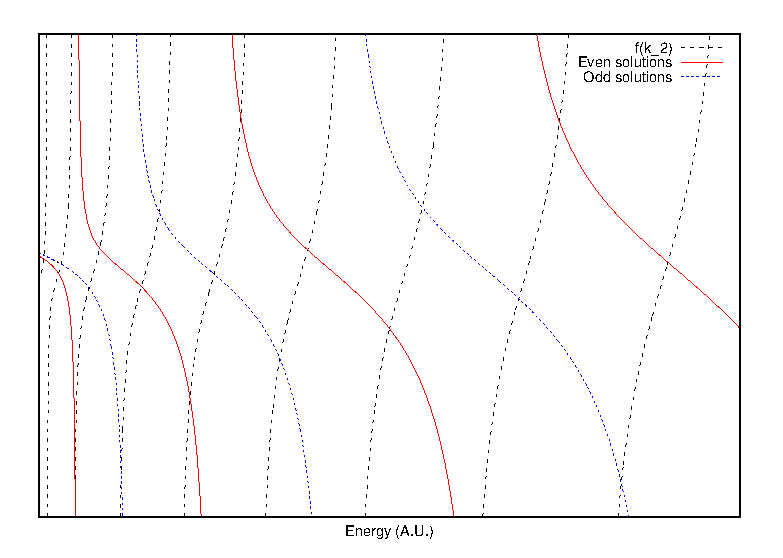
\includegraphics{graph_sol_ex_1_3.eps}
\caption{graphic solution of transcendental equation to get allowed energy values}
\label{graph_sol_ex_1_3}
\end{figure}

In fig. \ref{ex_1_3_ground_energies} we can see the intersections revealing the energies for the ground and first excited states. The intersection lower in energy is related to even solutions, while the other interesection is related to odd solutions. Therefore, the ground state is even while the first excited state is odd. The wavefunctions for ground and first excited states are presented in fig. \ref{ex_1_3_psi}.

\begin{figure}
\centering
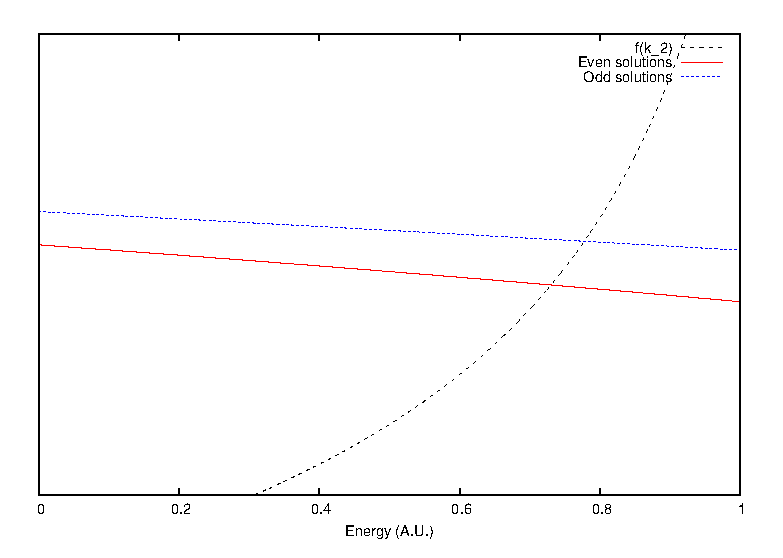
\includegraphics{ex_1_3_ground_energies.eps}
\caption{intersections revealing energies for the ground and first excited states}
\label{ex_1_3_ground_energies}
\end{figure}

\begin{figure}
\centering
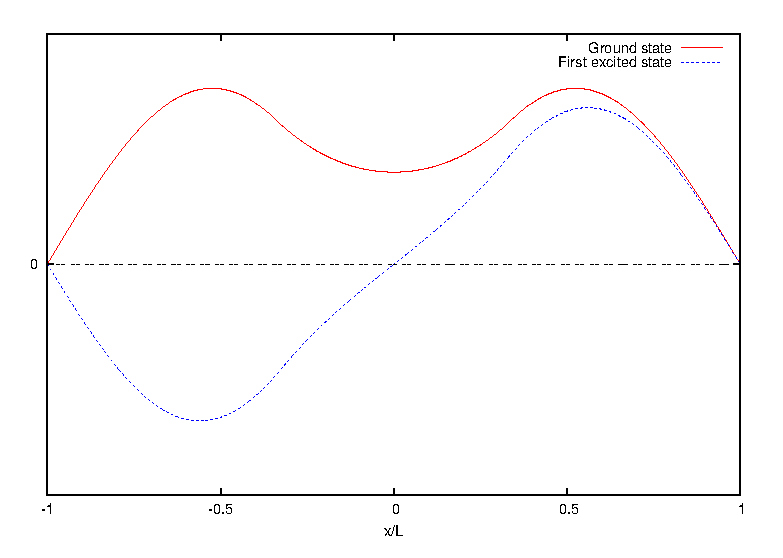
\includegraphics{ex_1_3_psi.eps}
\caption{wave functions for ground and first excited states}
\label{ex_1_3_psi}
\end{figure}

\section{Rabi pulses}

\subsection{Equation for \(C_{\pm}(t) \)}
The two-state problem is defined by the hamiltonian

\begin{equation}
H_0 = \frac{\hbar}{2} \omega \sigma_z
\end{equation}

plus a time-dependet perturbation

\begin{equation}
V(t) = v_o \frac{\hbar}{2} sin(\tilde{\omega} t) \sigma_x
\end{equation}

The eigenstates of \(H_0\) are \( \ket{\psi_+} \) and \( \ket{\psi_-} \), such that working in the interaction picture we have

\begin{equation}
\ket{\psi(t)} = c_+(t) \ket{\psi_+} + c_-(t) \ket{\psi_-}
\end{equation}

and the equation for the coefficients is (making the time dependence implicit)

\begin{equation}
i\hbar
  \begin{pmatrix}
    \dot{c}_- \\
    \dot{c}_+
  \end{pmatrix}
=
  \begin{pmatrix}
    V_{11} & V_{12}e^{i \omega_- t} \\
    V_{21}e^{i \omega_+ t} & V_{22}
  \end{pmatrix}
  \begin{pmatrix}
    c_- \\
    c_+
  \end{pmatrix}
\end{equation}

with

\begin{equation}
E_- = \bra{\psi_-} H_0 \ket{\psi_-} = -\frac{\hbar \omega}{2} = - E_+
\end{equation}

\begin{equation}
\omega = \omega_+ = \frac{E_+ - E_-}{\hbar} = -\omega_-
\end{equation}

Making the potential explicit we obtain

\begin{equation}
i\hbar
  \begin{pmatrix}
    \dot{c}_- \\
    \dot{c}_+
  \end{pmatrix}
=
  \begin{pmatrix}
    0 & v_o \frac{\hbar}{2} sin(\tilde{\omega} t) e^{i \omega_- t} \\
    v_o \frac{\hbar}{2} sin(\tilde{\omega} t) e^{i \omega_+ t} & 0
  \end{pmatrix}
  \begin{pmatrix}
    c_- \\
    c_+
  \end{pmatrix}
\end{equation}

from which we get the final system of differential equations for the coefficients

\begin{equation}
\label{eq:c_diff_eq}
  \begin{cases} 
      i\hbar \dot{c}_- = \frac{1}{2} \hbar v_0 sin(\tilde{\omega}t) e^{-i \omega t} c_+ = \frac{1}{4i} \hbar v_0 \left( e^{i(\tilde{\omega}-\omega)t} - e^{-i(\tilde{\omega}+\omega)t} \right) c_+ \\
      i\hbar \dot{c}_+ = \frac{1}{2} \hbar v_0 sin(\tilde{\omega}t) e^{i \omega t} c_- = \frac{1}{4i} \hbar v_0 \left( e^{i(\tilde{\omega}+\omega)t} - e^{-i(\tilde{\omega}-\omega)t} \right) c_-
   \end{cases}
\end{equation}

\subsection{Solution in rotating wave approximation}
Working with the rotating wave approximation, we have

\begin{equation}
\frac{\omega-\tilde{\omega}}{\omega} \ll 1 \quad \Rightarrow \quad \omega - \tilde{\omega} \ll \omega + \tilde{\omega}
\end{equation}

so we can neglect the terms of higher frequency in eq. \eqref{eq:c_diff_eq} to obtain

\begin{equation}
\label{eq:c_diff_eq_approx}
  \begin{cases} 
      i\hbar \dot{c}_- = \frac{1}{4i} \hbar v_0 e^{i(\tilde{\omega}-\omega)t} c_+ \\
      i\hbar \dot{c}_+ = - \frac{1}{4i} \hbar v_0 e^{-i(\tilde{\omega}-\omega)t} c_-
   \end{cases}
\end{equation}

Substituting the trial solution

\begin{equation}
\label{eq:trial_solution}
  \begin{pmatrix}
    c_- \\
    c_+
  \end{pmatrix}
=
  \begin{pmatrix}
    a_- e^{i\frac{\tilde{\omega} - \omega}{2}t} \\
    a_+ e^{-i\frac{\tilde{\omega} - \omega}{2}t}
  \end{pmatrix}
\end{equation}

into eq. \eqref{eq:c_diff_eq_approx} we get

\begin{equation}
  \begin{cases}
    a_- = \frac{i\hbar}{\gamma^*} \left( i\frac{(\tilde{\omega}-\omega)t}{2} a_+ + \dot{a}_+ \right) \\
    a_+ = \frac{i\hbar}{\gamma} \left( i\frac{(\tilde{\omega}-\omega)t}{2} a_- + \dot{a}_- \right) \\
  \end{cases}
\end{equation}

with \( \gamma = \frac{\hbar v_0}{4i} \).

Substituting the explicit expressions of \( a_- \) and \( a_+ \) into eq. \eqref{eq:trial_solution} and then plugging the result back into eq. \eqref{eq:c_diff_eq_approx} we get the second order differential equation

\begin{equation}
  \begin{cases}
    \ddot{a}_- = - \left( \frac{\gamma^2}{\hbar^2} + \frac{(\tilde{\omega}-\omega)^2}{4} \right) a_- \\
    \ddot{a}_+ = - \left( \frac{\gamma^2}{\hbar^2} + \frac{(\tilde{\omega}-\omega)^2}{4} \right) a_+ \\
  \end{cases}
\end{equation}

for which the solution will look like

\begin{equation}
a_+ \sim sin \left[ \left( \frac{\gamma^2}{\hbar^2} + \frac{(\tilde{\omega}-\omega)^2}{4} \right)^{\frac{1}{2}} t \right]
\end{equation}

Given the initial conditions

\begin{equation}
c_-(0) = 1, \quad c_+(0) = 0
\end{equation}

the solution for \( c_+(t) \) is

\begin{equation}
\label{eq:c+}
c_+(t) = e^{-i \frac{\tilde{\omega}-\omega}{2}t} sin \left[ \left( \frac{\gamma^2}{\hbar^2} + \frac{(\tilde{\omega}-\omega)^2}{4} \right)^{\frac{1}{2}} t \right]
\end{equation}

\subsection{Maximum transfer and unitary fidelity}
From eq. \eqref{eq:c+} we get

\begin{equation}
\label{eq:c+2}
|c_+(t)|^2 = \frac{\gamma^2 / \hbar^2}{\gamma^2 / \hbar^2 + (\tilde{\omega}-\omega)^2/4} sin \left[ \left( \frac{\gamma^2}{\hbar^2} + \frac{(\tilde{\omega}-\omega)^2}{4} \right)^{\frac{1}{2}} t \right]
\end{equation}

\begin{equation}
|c_-(t)|^2 = 1 - |c_+(t)|^2 
\end{equation}

It is easy to see that the probability of being found in \( \psi_+ \) is maximum for

\begin{equation}
\tilde{\omega} = \omega
\end{equation}

which is called "resonance condition". This is the situation for which the transfer is maximum and eq. \eqref{eq:c+2} becomes

\begin{equation}
\label{eq:c+2_resonance}
|c_+(t)|^2 = sin^2\left(\frac{\gamma}{\hbar}t\right)
\end{equation}

The fidelity is given by

\begin{equation}
F = |\braket{\psi(t)}{\psi_+}| = |c_+^*(t)| = |c_+(t)|
\end{equation}

and from eq. \eqref{eq:c+2_resonance} it is clear that it is maximum for

\begin{equation}
|c_+(t)|^2 = sin^2\left(\frac{\gamma}{\hbar}t\right) = 0 \quad \Rightarrow \quad t = \frac{\hbar \pi}{2 \gamma} (2n +1)
\end{equation}

\end{document}
